\chapter{Progetto Classificatore}
\label{progetto}

\todo{riscrivere}

%In questo capitolo si propone il progetto realizzato per raggiungere gli obiettivi preposti: la realizzazione di un classificatore basato sull'algoritmo di machine learning \textit{Random Forest} in grado di distinguere domini generati algoritmicamente da domini reali. Si è successivamente progettato un classificatore più raffinato basato su rete neurale in grado di superare le mancanze de precedente classificatore. A partire da tale sistema, si è passati alla progettazione di un sistema di \textit{adversarial learning} in grado di rafforzare il classificatore neurale: una \textit{Generative Adversarial Network} (abbr. \textit{GAN}) in grado di creare domini sintetici realistici da fornire successivamente al classificatore in fase di training (Figura~\ref{fig:intro}). Tale GAN è stata progettata a partire da un Autoencoder, il cui compito è mimare la distribuzione di un dataset fornito in input (Figura~\ref{fig:auttogan}).

\begin{figure}[p]
    \centering
	%\documentclass{standalone}
%\usepackage{tikz}

%\usetikzlibrary{shapes,arrows,fit,calc,positioning}
%\usetikzlibrary{backgrounds}
\tikzstyle{input} = [coordinate]
\tikzstyle{output} = [coordinate]
\tikzstyle{box} = [draw, rectangle, fill=white, rounded corners, thick, node distance=10em, text width=7em, text centered, minimum height=5em]
\tikzstyle{container} = [draw, rectangle, dashed, inner sep=1em, node distance=5em]
\tikzstyle{line} = [draw, thick, -latex']
%\begin{document}
\begin{tikzpicture}[auto, node distance=10em]
	\node [input](input){};
	\node [box, right of=input](clas){Classificatore};
	\node [box, below of=clas](gan){Generative Adversarial Network};
	\node [container, fit=(gan)](adv){};
	\node at (adv.south) [below,node distance=0 and 0] {Adversarial Learning};	
	\node [output, right of=clas](output){};
		
	
	\path [line] (input) -- node[near start](dataset){Dataset} (clas);
	\path [line] (dataset) |- (gan);
	\path [line] (gan) -- node[right]{Rinforzo} (clas);
	\path [line] (clas) -- (output)node[near end,name=out]{Decisione};
\end{tikzpicture}
%\end{document}
	\caption{Diagramma generale di progetto. \label{fig:intro}}
    \vspace{3cm}
    \centering
	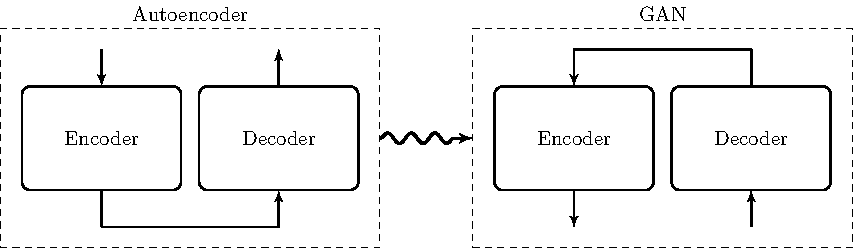
\includegraphics[width=\columnwidth]{figures/auttogan.tex}
	\caption{Schema generale della progettazione da Autoencoder a Gan. \label{fig:auttogan}}
\end{figure}

\newpage
\section{Classificatore Machine Learning}
\label{fig:classml}

\todo{rivedere nominazione del classificatore. rileggere capitolo}

La prima fase di questo studio è stata quella di progettare un classificatore in grado di separare efficacemente domini \textit{DGA} da domini reali basandosi unicamente sulle caratteristiche linguistiche dei domini: infatti, ad un esame preliminare, i domini \textit{DGA} presentano caratteristiche ben differenti dalle semplici frasi o parole che solitamente compongono i domini reali.
All'interno del classificatore, ogni albero dell'insieme è costruito a partire da un campione estratto con sostituzione dal \textit{training set}. In aggiunta, al momento della divisione del nodo durante la costruzione di un albero, la divisione scelta non è più la migliore soluzione tra tutte le \textit{features}. Al suo posto, la divisone che viene scelta è la migliore divisione all'interno di un \textit{subset} casuale tra tutte le \textit{features}. Come risultato di questa casualità, il \textit{bias} della foresta di solito aumenta leggermente (rispetto al \textit{bias} di un singolo albero non casuale) ma, a causa della media, la sua varianza diminuisce, di solito compensando l'aumento di \textit{bias}, quindi dando un modello generale migliore.

\subsection{Dataset}
\label{pro:randomforestdataset}
I \textit{dataset} di \textit{training} e \textit{testing} sono stati ricavati due fonti differenti: per quel che riguarda i domini reali si è fatto riferimento alla classifica dei domini più visitati al mondo fornita da \textit{Alexa Internet Inc.}~\cite{amazon:alexa} , per un totale di 1 milione di siti realmente esistenti; mentre grazie al repository fornito da~\cite{github:dgarepo} è stato possibile ottenere un \textit{dataset} esaustivo di esempi \textit{DGA} da diverse famiglie di \textit{malware} tra i quali ransomware come \textit{cryptolocker} e \textit{cryptowall}, trojans bancari come \textit{hesperbot}, e information stealers come \textit{ramnit}. Le tecniche DGA tradizionali variano in complessità da semplici approcci che estraggono caratteri casualmente a quelli che cercano di mimare la distribuzione di lettere o parole trovate nei domini reali. Il DGA di \textit{ramnit}, ad esempio, crea nomi di dominio usando una combinazione di moltiplicazioni, divisioni e resti a partire da un seme randomico. Agli antpodi, \textit{suppobox} crea domini concatenando due parole scelte in maniera pseudo-casuale da un piccolo dizionario Inglese.
In tabella~\ref{tab:dga} vengono mostrati alcuni esempi di domini generati algoritmicamente a seconda delle diverse famiglie di malware.
La maggior parte dei DGA opera a livello di singoli caratteri, mentre altre tipologie comuni come beebone hanno una struttura rigida, che produce domini come ns1.backdates13.biz e ns1.backdates0.biz.
Il DGA symmi produce domini vagamente pronunciabili tra i quali “hakeshoubar.ddns.net” estraendo una vocale o una consonante casualmente per ogni indice pari e successivamente estraendo l’opposto all’indice successivo oltre che ad aggiungere un dominio di primo e secondo livello al termine della stringe come .ddns.net
La distribuzione dei singoli caratteri (unigrammi) per 4 famiglie di DGA e Alexa sono mostrate di seguito. La distribuzione di cryptolocker e ramnit sono entrambe uniformi all’interno dello stesso range. Si tratta di una caratteristica attesa in quanto entrambi sono generati tramite una serie di moltiplicazioni, divisioni e resti basati su di un singolo seme. Suppobox, d’altro canto presenta caratteristiche interessanti in quanto genera unigrammi simili per distribuzione ad Alexa. 

\begin{table}[p]
    \centering
    \resizebox{0.4\textwidth}{!}{%
    \begin{tabular}{ l|l }
        corebot & ep16g6gjwfixyhs8gfy.ddns.net \\
 		& ev5texifc43nebil3pk.ddns.net \\
 		& gf7bm4163fmjkje.ddns.net \\
		cryptolocker & agryjvdaabkyt.ru \\
 		& pwitjnqgjfaqm.org \\
 		& dhhubfepcdgfv.co.uk \\ 
		dircrypt & hedhryendqlss.com \\
 		& lgnggnlufbtyjpnvct.com \\
 		& tzrbdmhoumoy.com \\
		kraken v2 & fwulvdmdytm.com \\
 		& gybuisybe.cc \\
 		& gyinkvye.net \\
		lockyv2 & btlwubflhfllshn.info \\
 		& cpgcjsysfwuwa.click \\
 		& jlbroeji.biz \\
		pykspa & gqjgflhop.net \\
 		& gqumcwaa.org \\
 		& jpivjh.net \\
		qakbot & fgfifkyfut.info \\
 		& flzuzsaekkipatbtet.biz \\
 		& owpbsjekk.com \\
		ramdo & kugmywaaiymaegiq.org \\
 		& ocywskaagmmqscoc.org \\
 		& uomywsaaqggiwouo.org \\
		ramnit & byqdmekgd.com \\
 		& dpmdbwwcmpk.com \\
 		& gkkcoufektvhiqr.com \\
		simda & gatyfusyfi.com \\
		& lyvyxoryco.com \\
 		& puvyxilomo.com \\
    \end{tabular}
    }

\caption{Esempi di domini generati algoritmicamente da Malware. \label{tab:dga}}
\end{table}


A partire da tale \textit{dataset} combinato si è proceduto alla creazione di un classificatore binario che fosse in grado di distinguere domini reali da domini generati algoritmicamente. 
Il passo seguente  stato creare una serie di \textit{features} che fossero in grado di descrivere le caratteristiche linguistiche dei domini presi in esame.


\begin{figure}[!bp]
    \centering
    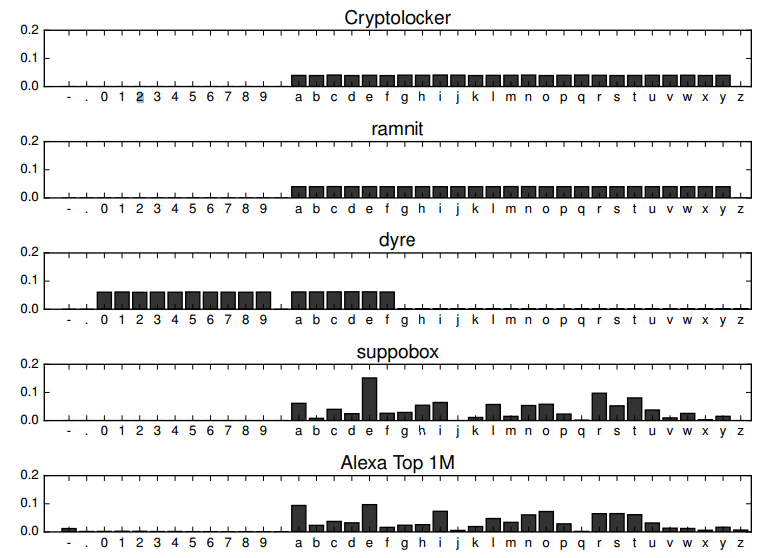
\includegraphics[width=\columnwidth]{figures/chardistr.png}
    \caption{Distribuzione dei singoli caratteri in \textit{cryptolocker, ramnit, dyre}, \textit{suppobox} (dictionary-based DGA) ed il primo milione di domini più visitati secondo Alexa~\cite{amazon:alexa}.
\textit{fonte:}~\cite{deepdga}. \label{fig:Chardistr}}
\end{figure}


Per raggiungere tale obiettivo si è fatto riferimento a ricerche già esistenti:~\cite{180232}~\cite{Yadav:2010:DAG:1879141.1879148}~\cite{Yadav:2012:DAG:2428696.2428722}~\cite{Schiavoni2014}. Di seguito viene illustrato l'insieme di tali \textit{features}:

\subsection{Features}
\label{randomforestinterno}

\begin{itemize}

\item \textbf{Rapporto tra caratteri significativi}. Modella il rapporto dei caratteri della stringa $p$ che formano una parola significativa all'interno del dizionario Inglese. Un valore basso indica la presenza di algoritmi automatici. In dettaglio, si divide $p$ in $n$ sotto-parole significative $w_i$ di almeno $3$ caratteri: $|wi| \ge 3$ cercando di lasciare fuori meno caratteri possibili: 

\[R(d) = R(p) = \frac{max(\sum_{i=1}^n |wi|)}{\left | p \right |}\] 

Se $p = \text{facebook}$, $R(p) = \frac{(|\text{face}| + |\text{book}|)}{8} = 1$ allora il dominio è composto completamente da parole significative, mentre $p = \text{pub03str}$, $R(p) = \frac{|\text{pub}|}{8} = 0.375$. 

    

\item \textbf{Punteggio di normalità degli n-grammi}: Questa classe di \textit{features} modella la pronunciabilità di un nome di dominio rispetto la lingua Inglese. Più la combinazione di fonemi del dominio è presente  all'interno del Dizionario Inglese più tale dominio è pronunciabile. Domini con un basso numero di tali combinazioni sono probabilmente generati algoritmicamente. Il calcolo avviene estraendo lo n-gramma di $p$ di lunghezza $n \in \left \{1, 2, 3, 4, 5 \right \}$ e contando il numero di occorrenze di tale n-gramma all'interno del Dizionario Inglese. Tali \textit{features} sono quindi parametriche rispetto ad n:
 
\[S_n(d) = S_n(p) \:= \frac{\sum_{\text{n-gramma t in p}} count(t)}{\left | p \right | - n + 1}\] 

dove $count(t)$ sono le occorrenze dello n-gramma nel dizionario. Ad esempio $S_2(facebook) = fa_{109} + ac_{343} + ce_{438} + eb_{29} + bo_{118} + oo_{114} + ok_{45} = 170.8$

       
\item \textbf{Rapporto tra caratteri numerici} Questa \textit{feature} rappresenta il rapporto tra i caratteri numerici presenti all'interno del nome di dominio rispetto la lunghezza totale della parola. Molte famiglie di \textit{malware} utilizzano \textit{DGA} che generano domini tramite una distribuzione uniforme di caratteri alfabetici minuscoli e numeri, questo porta a domini generati algoritmicamente che presentano una maggior presenza di numeri al loro interno rispetto ai domini reali.


\item \textbf{Rapporto tra vocali e consonanti} Questa \textit{feature} modella il rapporto tra vocali e consonanti all'interno del nome di dominio.


\item \textbf{Lunghezza del nome di dominio} Questa \textit{feature} calcola la lunghezza del dominio. Molte famiglie di \textit{malware} utilizzano \textit{DGA} che generano domini di lunghezza costante, generalmente molto lunghi rispetto ai domini reali.
	
\end{itemize}

L'implementazione di tali \textit{features} ha permesso di ottenere un \textit{dataset} in grado di modellare le caratteristiche linguistiche dei nomi di dominio mostrati al capitolo~\ref{randomforestdataset}. Da tale spunto è partita la fase iniziale di \textit{testing} 

\subsection{Architettura Interna}
La scelta della tipologia di architettura da utilizzare per il classificatore è stata ridotta a tre modelli di classificazione differenti: 
\begin{itemize}
\item \textbf{Random Forest}~\cite{randomforest}: un metodo di \textit{ensemble learning}~\cite{ensemble} supervisionato per la classificazione che opera tramite la costruzione di un insieme di alberi decisionali durante la fase di training ed emette la classe che rappresenta la moda statistica delle classi individuate dai singoli alberi. Formalmente è definita dalla seguente funzione:
Per un punto $x$, sia $v_j(x)$ il nodo terminale a  cui $x$ è assegnato durante la discesa dell'albero $T_j$ $\left(j=1,2,\dots,t\right)$.
Sia indicata da $P(c|v_j(x))$ la probabilità a posteriori che $x$ appartenga alla classe $c (c = 1,2,\dots,n)$ come:
\[P(c|v_j(x) = \frac{P(c,v_j(x))}{\sum_{l=1}^n P(c_t,v_j(x))}\]
Tale probabilità può essere stimata dalla frazione di punti di classe $c$ rispetto a tutti i punti che sono assegnati a $v_j(x)$. 
La funzione di discriminazione è definita da:
\[g_c(x) = \frac{1}{t}\displaystyle\sum_{j=1}^{t} \hat{P}(c|v_j(x))\]
e la regola decisionale è assegnare $x$ alla classe $c$ per cui $g_c(x)$ è massimo.

\item \textbf{Support Vector Machine}~\cite{svm}:  un metodo di apprendimento supervisionato per la classificazione basati sul concetto di piani decisionali, che definiscono i limiti di decisione. L'algoritmo costruisce un iperpiano o un set di iperpiani in uno spazio multidimensionale, usato per la classificazione. Un esempio è mostrato in figura~\ref{fig:svm}

Formalmente è definito da:
Dati i vettori di training $x_i \in \mathbb{R^p}, i=1,\dots,n$ in due classi e un vettore $y \in \left\lbrace1,-1\right\rbrace^n$ il classificatore risolve il problema:
\begin{align*}
& \min_{\omega,b,\zeta} \frac{1}{2} \omega^T \omega + C  \displaystyle\sum_{i=1}^n \zeta_i \\
&\text{soggetto a } y_i(\omega^T \phi(x_i) + b) \geq 1 - \zeta_i, \\
&\zeta_i \geq 0, i =1,\dots,n
\end{align*}
il cui duale è definito da:
\begin{align*}
& \min_{\alpha} \frac{1}{2} \alpha^T Q\alpha - e^T \alpha \\
&\text{soggetto a } y^T \alpha = 0 \\
& 0 \leq \alpha_i \leq C, i = 1, \dots, n
\end{align*}
dove $e$ è un vettore di 1, $C > 0$ è il limite superiore, $Q$ è una matrice $n \times n$ positiva semidefinita, $Q_{ij} \equiv y_iy_jK(x_i,x_j)$, dove $K(x_i,x_j) = \phi(x_i)^T \phi(x_j)$ è il kernel. I vettori di training sono implicitamente mappanti in uno spazio dimensionale più grande dalla funzione $\phi$. 
La funzione di decisione è:
\[ sgn \left(\displaystyle\sum_{i=1}^n y_i \alpha_i K(x_i,x) + \rho \right) \] 

\begin{figure}[!bp]
    \centering
    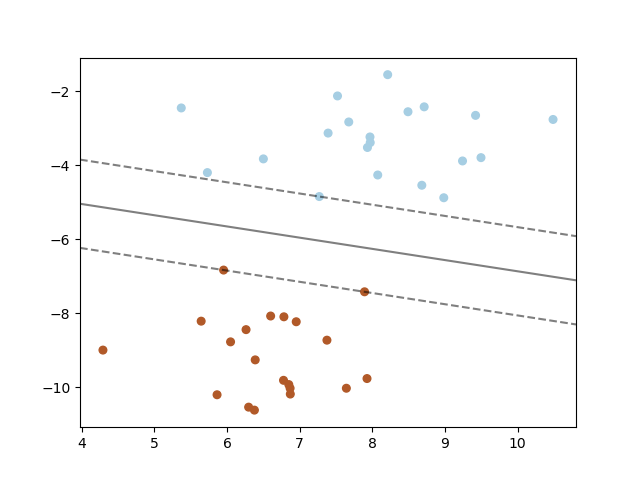
\includegraphics[width=\columnwidth]{figures/svm.png}
    \caption{Esempio di iperpiano di una SVM. \label{fig:Chardistr}}
\end{figure}

\item \textbf{Naive Bayes}: Metodo di classificazione supervisionata basati sul teorema di Bayes con un assunto "\textit{naive}" di indipendenza tra ogni coppia di feature. Data una variabile di classe $y$ e un vettore di features indipendenti $x_1 \dots, x_n$ il teorema di Bayes dimostra la seguente relazione: 

\[P\left(y|x_1,\dots,x_n\right) = \frac{P(y)P(x_1,\dots,x_n|y)}{P(x_1,\dots,x_n)}\]
 
Siccome $P(x_1,\dots,x_n)$ è una costante data in ingresso è definita la seguente regola di classificazione:
 
 \[\hat{y} = arg,\max_{y}P(y)\displaystyle\prod_{i=1}^n P(x_i|y)\]
 
\end{itemize}

Il classificatore è stato implementato e testato con i tre modelli. Si confrontino i risultati all'interno del capitolo~\ref{risultati}.

\subsection{Output}
\label{randomforestoutput}
L'obiettivo di tale classificatore è quello di riuscire a separare in maniera efficace i domini reali da quelli generati algoritmicamente. Durante la fase di sperimentazione il classificatore si è rivelato efficace rispetto la maggior parte delle famiglie di \textit{DGA}; tuttavia il caso particolare della famiglia \textit{suppobox}~\cite{geffner2013end} ha messo in particolare difficoltà il classificatore in quanto tale algoritmo genera domini in maniera pseudo-casuale, concatenando due parole a partire da un \textit{subset} di 384 parole provenienti dal dizionario inglese. Tale caratteristica fa si che le \textit{features} linguistiche estratte da questa famiglia di \textit{malware} siano molto simili a quelle presenti nei domini reali. In tabella~\ref{tab:suppobox} sono mostrati alcuni esempi di domini generati da Suppobox.


\begin{table}[!htbp]
    \centering
    \begin{tabular}{|l|}
        \hline
        Suppobox
        \\
        \hline
        \hline
       	increaseinside.net \\
		wouldinstead.net \\
		rememberinstead.net \\
		wouldexplain.net \\
		rememberexplain.net \\
		wouldbright.net \\
		rememberbright.net \\
		wouldinside.net \\
		rememberinside.net \\
        \hline
    \end{tabular}
    \caption{Esempio di domini generati da Suppobox. \label{tab:suppobox}}
\end{table}

A partire da questo risultato si scelto di procedere con la progettazione di un classificatore neurale in grado di superare tale problematica.

\newpage
\section{Classificatore Neurale}
\label{classificatorenn}
Questo classificatore neurale nasce con l'intento di superare le difficoltà incontrate dal precedente classificatore basato su \textit{Random Forest}, utilizzando le caratteristiche delle reti neurali, in grado di estrarre \textit{features} a partire dai dati grezzi. Si è scelto di partire dall'architettura di tipo \textit{Multilayer Perceptron} con l'obiettivo di ottenere risultati migliori rispetto al caso mostrato nella sezione precedente.

I passi del progetto sono stati la codificazione dei domini in valori numerici, l'individuazione di una architettura ottimale per classificare i dati in esame ed un'ultima fase di \textit{tuning} degli iperparametri della rete neurale. 

\subsection{Dataset}
\label{classificatorenninput}
A partire dal \textit{dataset} creato per il precedente caso, si è deciso di convertire direttamente i nomi di dominio alfanumerici in vettori numerici, mappati secondo il dizionario di tutti i caratteri ammessi~\cite{icann} (lettere minuscole a-z, numeri 0-9, tratto d'unione "-" ). L'obiettivo è quello di fornire al classificatore neurale in questione una rappresentazione il più possibile aderente ai dati reali, senza l'ausilio di \textit{features} ingegnerizzate a priori, lasciando così la libertà alla rete neurale di estrarre le caratteristiche più appropriate per la distinzione dei domini. Come scelta progettuale si è deciso di limitare la dimensione dei domini a 15 caratteri per ognuno, in modo da ottenere un \textit{dataset} di dimensioni fissate e sopperire alle differenti lunghezze di ogni dominio tramite un semplice \textit{padding} di zeri in testa ad ogni stringa codificata.

Assieme ai dati codificati è stato generato un vettore di \textit{target} nel quale viene indicato da 0 o da 1 se il dominio in esame è di tipo reale o generato algoritmicamente. L'obiettivo quindi è di attuare un classificatore binario in grado di prevedere correttamente a quale categoria appartiene un dominio esaminato 

\subsection{Architettura Classificatore Neurale}
\label{classificatorenninterno}
L'architettura scelta in prima fase è stata quella del \textit{Multilayer Perceptron} \textit{(abbr. MLP)}, una tipologia di rete neurale \textit{feedforward} tipicamente formata da almeno tre livelli di nodi. Ad esclusione del livello di \textit{input} i livelli del MLP utilizzano  funzioni di attivazione non lineari che permettono di eseguire distinzioni tra dati non linearmente separabili. Considerando una rete formata da $m$ neuroni,  se si considera $d$ come numero di input, si avrà il seguente output

\[y_j=y\left( \sum_{i=0}^d w_{ji}x_i \right)\]


nel quale $x_i$ sono gli input e $w_{ji}$ sono i pesi di ogni input combinati con ogni output. 

Nel caso in esame è stata utilizzata per i livelli interni la funzione di attivazione \textit{Rectifier Linear Unit} (ReLU)~\cite{relu} definita dalla funzione sottostante e mostrato in figura~\ref{fig:relu}

\[f(x) = x^+ = max(0,x)\]

\begin{figure}[htb]
    \centering
    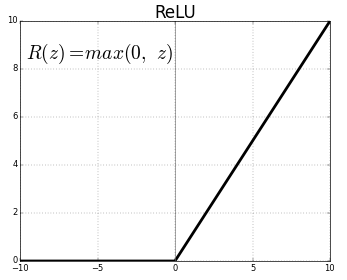
\includegraphics[width=0.7\columnwidth]{figures/relu.png}
    \caption{\textit{fonte:}~\cite{relufig}.\label{fig:relu}}
\end{figure}

dove $x$ rappresenta l'\textit{input} del neurone. 
I vantaggi di tale funzione sono una migliorata \textit{performance} rispetto ad altre funzioni similari come \textit{tanh} e \textit{sigmoid} per quel che riguarda la convergenza della discesa stocastica del gradiente. 

Per quel che riguarda la funzione di attivazione del livello di \textit{output} si è scelta la funzione \textit{sigmoidea}, definita dalla formula 

\[P(t) = \frac{1}{1+e^{-t}}\]

\begin{figure}[htb]
    \centering
    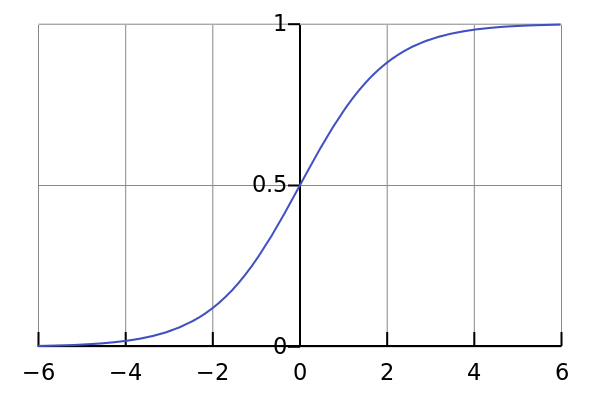
\includegraphics[width=0.7\columnwidth]{figures/sigmoid.png}
    \caption{\textit{fonte:}~\cite{fig:sigmoid}\label{fig:sigmoid}}
\end{figure}

La struttura finale del \textit{MLP} in esame è stata raggiunta dopo una serie di test sperimentali in cui si sono messi a confronto tre modelli differenti di per numero di neuroni all'interno degli \textit{hidden layer}: 
\begin{itemize}
\item un modello ridotto composto da un layer di input con un numero di neuroni pari alla dimensione delle stringhe codificate, un layer intermedio di dimensione dimezzata rispetto al precedente ed il layer finale di uscita di dimensione 1 per attuare la classificazione binaria, oggetto di studio.

\item un modello allargato composto da un layer di input con un numero di neuroni pari alla dimensione delle stringhe codificate, due layer intermedi di dimensioni moltiplicate di diversi ordini rispetto al layer iniziale ed un layer finale di dimensione 1.

\item un modello intermedio composto da un layer di input con un numero di neuroni pari alla dimensione delle stringhe codificate, due layer intermedi di dimensioni comprese tra i valori ottenuti dal modello ridotto ed il modello allargato ed un layer finale di dimensione 1. 

\end{itemize}

I tre modelli sono stati messi a confronto in fase sperimentale, dovendo procedere ad una fase di tuning dei parametri che compongono il modello intermedio in quanto non è possibile in maniera automatica determinare quali siano i parametri ottimali per il MLP utilizzato nel caso in esame.

\begin{figure}[htbp]
	\centering
	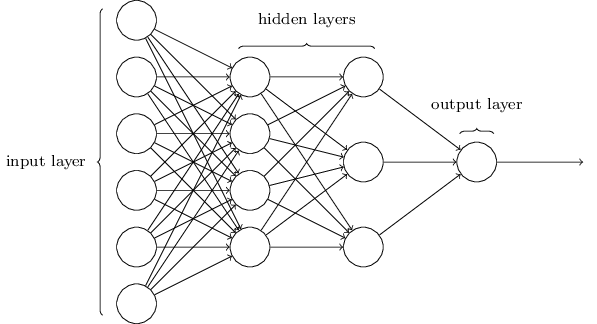
\includegraphics[width=\columnwidth]{figures/mlp-network.png}
	\caption{Schema generico di un Multilayer Perceptron \label{mlp}}
\end{figure}

\subsection{Output}
\label{classificatorennoutput}
L'intento della rete neurale proposta è quello di classificare autonomamente domini reali da domini generati algoritmicamente, con l'obiettivo di superare le fragilità del classificatore precedente (\ref{fig:classml}) ed avere una linea di confronto affidabile per lo \textit{step} di lavoro successivo: l'introduzione di un sistema di \textit{adversarial learning} che possa rafforzare tale classificatore. 

\newpage
\chapter{Progetto Adversarial Learning}
\label{adv}
Ricerche precedenti hanno dimostrato che molti modelli di machine learning, incluse le reti neurali, sono vulnerabili agli \textit{adversarial examples}~\cite{1312.6199}, ~\cite{1412.6572}. In particolare la ricerca proposta in~\cite{1412.6572} introduce il metodo del \textit{fast gradient sign} per scoprire \textit{adversarial examples} perturbando un campione noto $x$ con una piccola quantità definita  
\[\Delta x =  \in sign(\nabla_x J(\theta,x,y))\] 
dove $\theta$ rappresenta i parametri del modello e $J$ il costo necessario a classificare $x$ come $y$.
Separatamente~\cite{1406.2661} propone l'uso di \textit{Generative Adversarial Network (abbr. GAN})  come \textit{framework} in grado di generare campioni artificiali provenienti dalla stessa distribuzione del training set.
Le \textit{GAN} incorporano due modelli: un generatore ed un discriminatore i quali competono in una serie di turni antagonisti. All'interno del contesto del lavoro presentato in questo elaborato, il generatore impara a creare nuovi domini artificiali mentre il discriminatore impara a distinguere tali domini artificiali da quelli reali. L'intento di tale lavoro è usare la \textit{GAN} per produrre domini artificiali realistici e di conseguenza incrementare la precisione del classificatore presentato nella sezione precedente attraverso l'\textit{adversarial training}. I presupposti progettuali di questo elaborato sono ispirati alla ricerca presentata in~\cite{deepdga}.

\newpage
\section{Autoencoder}
\label{autoencoder}
Il punto di partenza per il lavoro di progettazione di una \textit{GAN} è stato l'implementazione di un \textit{Autoencoder} funzionante.  Un \textit{Autoencoder} è un modello di rete neurale non supervisionata con lo scopo di riprodurre il proprio input passando attraverso una rappresentazione codificata, generalmente a dimensione inferiore~\cite{MAL-006}~\cite{Liou:2008:MWP:1411851.1412074}. Si supponga di avere un set di training $\left\{ x^{(1)}, x^{(2)}, x^{(3)}, \ldots \right\}$ dove $x^{(i)} \in \mathbb{R}^n$. L'obiettivo di un autoencoder generico è \[y^{(i)} = x^{(i)}\] cercando di imparare una funzione che approssima x \[h_{W,b}(x) \approx x\]. Un \textit{autoencoder} tipicamente consiste in due macro-componenti:
\begin{itemize}
\item funzione \textbf{Encoder} $h = f(x)$ la quale trasforma l'input una rappresentazione codificata (generalmente a dimensione minore)
\item funzione \textbf{Decoder} $r = g(h)$ in grado di ricostruire l'input a partire dalla rappresentazione codificata. 
\end{itemize}

\begin{figure}[htb]
    \centering
	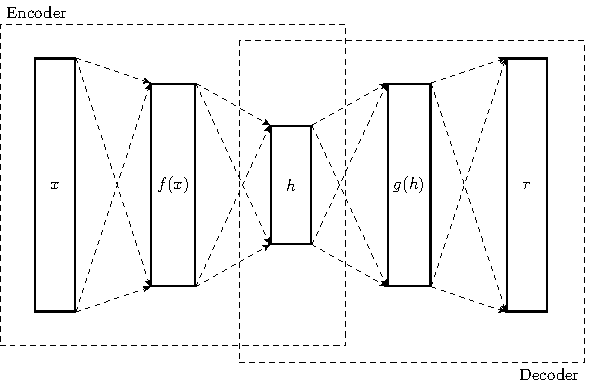
\includegraphics[width=\columnwidth]{figures/autoencoder_general.tex}
	\caption{Struttura generica di un autoencoder, il quale mappa l'input $x$ in un output $r$ attraverso una rappresentazione codificata $h$.
\label{fig:autoencodergen}}
\end{figure}

Tuttavia il reale obiettivo di un \textit{autoencoder }non è quello di imparare perfettamente a riprodurre l'input fornito (in quanto sarebbe un'operazione priva di utilità), bensì vengono introdotti vincoli che ne limitano la capacità di riproduzione ad una sola approssimazione dei dati di ingresso. Grazie a tali vincoli il modello è obbligato a dare priorità agli aspetti fondamentali dell'input, imparandone le proprietà principali. L'obiettivo di tale implementazione nel contesto di questo elaborato è poter cogliere le caratteristiche fondamentali che compongono i domini reali, per poterli riprodurre al meglio all'interno della \textit{GAN} e generare domini simili a quelli reali a partire da rumore casuale.

\subsection{Dataset Autoencoder}
\label{datasetautoencoder}
Il \textit{dataset} utilizzato per il training di tale \textit{autoencoder} è lo stesso mostrato nella sezione~\ref{classificatorenninput}, in cui i domini sono mappati in vettori numerici, secondo il dizionario di caratteri ammissibili per i domini. Durante la fase di implementazione si è reso necessario un ulteriore \textit{step} di \textit{preprocessing}: i domini codificati in sequenze di valori interi sono stati ulteriormente codificati tramite il \textit{one hot encoding}~\cite{onehot} in modo da formare un tensore 2D per ogni dominio, in cui ogni riga è formata da sequenze di bit a 0 tranne il carattere nella posizione indicata dal dizionario, il quale è indicato ad 1. I domini così codificati vengono trattati come una sequenza temporale, in cui ogni \textit{step} è caratterizzato da un vettore nel quale è indicato a 1 quale carattere del dizionario $\mathbb{V}$ vi è rappresentato. 

Questo ulteriore passaggio è diventato necessario durante l'implementazione della \textit{GAN}, in modo da poter utilizzare il tensore di output del \textit{decoder} come ingresso per l'\textit{encoder}.


\subsection{Architettura Autoencoder}
\label{archautoencoder}
L'architettura dell'\textit{encoder} in esame è ispirato al lavoro mostrato in~\cite{1508.06615} mentre il \textit{decoder} è approssimativamente una immagine speculare dell'\textit{encoder}.

Al domini codificati come indicato nella sezione precedente, vengono applicati dei filtri convoluzionali con l'obiettivo di catturare n-grammi significativi all'interno dei domini reali. Il layer successivo di concatenazione assembla l'output dei diversi filtri in un tensore di dimensione ridotta rispetto all'input iniziale e lo passa ad una LSTM la quale accumula stato lungo la sequenza di caratteri e ritorna in uscita il dominio codificato in forma di vettore mono-dimensionale.

Il \textit{decoder} è lascamente l'inverso del processo di codifica: il dominio codificato dato in input viene ripetuto un numero di volte equivalente alla lunghezza massima di nome di dominio decisa a priori e passato ad una LSTM. La sequenza di emissioni da parte del layer LSTM viene fornita agli stessi filtri convoluzionali presenti all'interno dell'\textit{encoder}. Questo risulta in un vettore $\mathbb{V}$-dimensionale per ogni elemento della sequenza che compone il dominio.
Lo step finale consiste di un dense layer con distribuzione temporale che agisce come regressore multinomiale. A causa dell'attivazione \textit{softmax} attuata sul \textit{dense layer}, l'output del decoder rappresenta una distribuzione multinomiale dei caratteri di $\mathbb{V}$ per ogni step temporale, la quale può essere campionata per produrre un nuovo nome di dominio contenente le caratteristiche principali dei nomi di dominio usati in input.

In figura~\ref{fig:autoencoder1} è mostrata la struttura di massima dell'autoencoder. Di seguito vengono illustrati in dettaglio le principali componenti che compongono l'\textit{autoencoder}. 

\begin{figure}[!p]
    \centering
	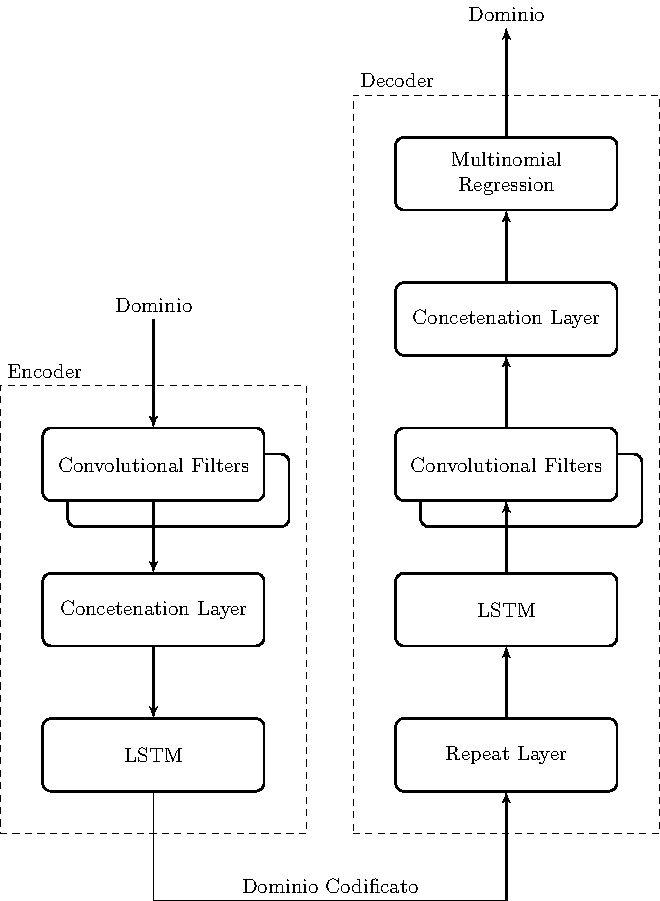
\includegraphics[width=\columnwidth]{figures/autoencoder.tex}
	\caption{Struttura dell'\textit{autoencoder} in esame. L'input in ingresso dato dai domini viene codificato attraverso l'\textit{encoder} e dato in ingresso al \textit{decoder} che ne genera una approssimazione.
\label{fig:autoencoder1}}
\end{figure}

\newpage
\section{Encoder}
\label{encoder}
La composizione interna dell'\textit{encoder} è formata da una Rete Convoluzionale accoppiata ad una LSTM. A differenza del lavoro proposto in~\cite{deepdga}, si è voluto mantenere la composizione dell'autoencoder il più semplice possibile, in quanto la trasformazione in \textit{GAN} ed il suo \textit{tuning} in fase di \textit{training} è notoriamente difficoltoso in presenza di molti parametri. In Figura~\ref{fig:encoder} viene mostrata la struttura semplificata dell'encoder.

\begin{figure}[!bp]
    \centering
	%\usetikzlibrary{shapes,arrows,fit,calc,positioning}
%\usetikzlibrary{backgrounds}
\tikzstyle{box} = [draw, rectangle, fill=white, rounded corners, thick, node distance=5em, text width=7em, text centered, minimum height=2.5em]
\tikzstyle{container} = [draw, rectangle, dashed, inner sep=1em, node distance=5em]

\tikzstyle{line} = [draw, thick, -latex']

\begin{tikzpicture}[auto]
	\node [box] (conv) {Convolution Layer};
	\node [box, below of=conv] (batch) {Batch Normalization};
	\node [box, below of=batch](leaky) {Leaky ReLU activation};
	\node [box, below of=leaky](dropout) {Dropout};
	\node [box, below of=dropout](pooling){Average Pooling};

	
	\node [box, right of=conv, node distance=12em] (conv2) {Convolution Layer};
	\node [box, below of=conv2] (batch2) {Batch Normalization};
	\node [box, below of=batch2](leaky2) {Leaky ReLU activation};
	\node [box, below of=leaky2](dropout2) {Dropout};
	\node [box, below of=dropout2](pooling2){Average Pooling};
	
	\node [draw=none, above of=conv](invis4){};
	\node [draw=none, above of=conv2](invis5){};
	\node [draw=none, fit=(invis4)(invis5)](invis6){};
	\coordinate[above of=invis6,node distance=3em](begin_enc);
	\node at (begin_enc.north) [above,node distance=0 and 0] (input){Dominio};

	\node [draw=none, below of=pooling](invis){};
	\node [draw=none, below of=pooling2](invis2){};
	\node [draw=none, fit=(invis)(invis2)](invis3){};
	
	\node[box,below of=invis3, node distance=3em](conc){Concatenation Layer};
	\node[box,below of=conc](lstm){LSTM};
	\coordinate[below of=lstm,node distance=3em](end_enc);
	\node at (end_enc.south) [below,node distance=0 and 0] (output){Dominio Codificato};

	\node [container, fit=(conv)(pooling)](cnn){};
	\node [container, fit=(conv2)(pooling2)](cnn2){};
	\node at (cnn.north west) [above right,node distance=0 and 0] {Convnet};
	\node at (cnn2.north east) [above left,node distance=0 and 0] {Convnet};

	\path [line] (conv) -- (batch);
	\path [line] (batch) -- (leaky);
	\path [line] (leaky) -- (dropout);
	\path [line] (dropout) -- (pooling);
	\path [line] (pooling) |- (conc);

	\path [line] (conv2) -- (batch2);
	\path [line] (batch2) -- (leaky2);
	\path [line] (leaky2) -- (dropout2);
	\path [line] (dropout2) -- (pooling2);
	\path [line] (pooling2) |- (conc);
	
	\path [line] (conc) -- (lstm);
	\path [line] (lstm) -- (end_enc);
	
	\path [line] (begin_enc) -| (conv);
	\path [line] (begin_enc) -| (conv2);
\end{tikzpicture}

	\caption{Struttura dell'\textit{encoder}.
\label{fig:encoder}}
\end{figure}

\subsection{Rete Convoluzionale}
Una Rete Convoluzionale è un modello di rete neurale usato generalmente per classificazione di immagini, in alternativa ai layer densamente connessi. Il vantaggio nell'uso delle reti convoluzionali è la capacità di quest'ultime di memorizzare pattern locali all'interno dello spazio di input mentre layer densamente connessi sono in grado di riconoscere solo pattern globali. Nel caso in esame si sono applicati due filtri convoluzionali in parallelo, con l'obiettivo di cogliere pattern locali all'interno dei domini, ovvero n-grammi significativi da poter replicare. Generalmente i filtri convoluzionali lavorano su di un tensore 3-dimensionale, chiamato \textit{feature map}, avente due assi spaziali ("altezza" e "larghezza") ed un asse di profondità; nel caso di riconoscimento di immagini tali assi corrispondono alle dimensioni dell'immagine di input ed al numero dei canali colore. Nel caso in esame si sono trattati di input tridimensionali ad altezza 1, larghezza equivalente alla dimensione massima dei domini nel dataset e canale di dimensione 1. L'operazione di convoluzione estrae frammenti dalla \textit{feature map} di input ed applica una trasformazione a tutti i frammenti, generando una \textit{output feature map} la quale è ancora in forma di tensore 3D, di dimensione ridotta, contenente sull'asse della profondità i valori dei \textit{filtri}. I filtri codificano determinati aspetti caratteristici dell'input, analizzando l'input in una "finestra" di dimensione fissata che scorre lungo la sequenza; ad ogni passo il filtro estrae il sotto-tensore 3-dimensionale per trasformarlo(tramite un prodotto tensore con una matrice di pesi (chiamato \textit{convolutional kernel}) in un vettore 1D di dimensione fissata. L'insieme di vettori vengono riassemblati in un tensore 3D con altezza e larghezza identiche alle precedenti e l'inseme di features come terzo asse. In figura~\ref{fig:cnn} è possibile vedere un diagramma del funzionamento di una rete convoluzionale.

\begin{figure}[!htbp]
    \centering
	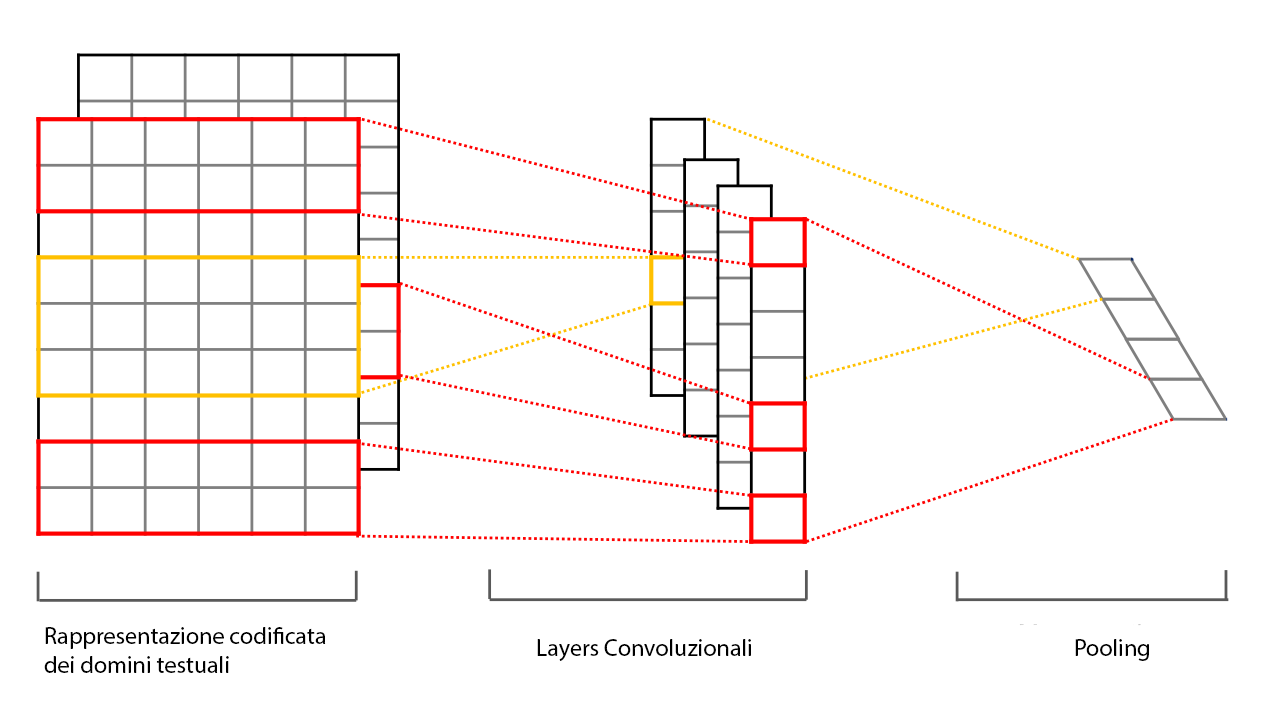
\includegraphics[width=\columnwidth]{figures/CNN.png}
	\caption{Funzionamento di una Convolutional Neural Network,\textit{ fonte}~\cite{fig:cnnfonte}.
\label{fig:cnn}}
\end{figure}


\subsection{Pooling}
Parte integrante di una rete convoluzionale è il livello di \textit{pooling}, in cui le features più importanti del livello precedente vengono ridotte in un tensore di dimensione inferiore, secondo il valor medio all'interno della \textit{feature map}. La decisione di utilizzare average pooling anziche max pooling è stata presa a causa dell'elevata instabilità intrinseca alle GAN, per le quali max pooling è un fattore contribuente. 

\subsection{Concatenazione}
Il layer aggiuntivo di \textit{concatenazione} funge permete di formare un unico vettore mono-dimensionale in grado di fornire le caratteristiche principali dei domini analizzati.

\subsection{Long Short-term Memory}
Seconda fase della sottorete Encoder è la presenza di una Long Short-term Memory Network \textit{(abbr LSTM)}~\cite{LSTM}. Si tratta di un modello di \textit{Recurrent Neral Network (abbr. RNN)} particolare, in grado di apprendere dipendenze a lungo termine all'interno di una sequenza temporale che nasce con l'intento di superare le principale problematiche delle RNN semplici, le quali non sono in grado di gestire dipendenze a lungo termine all'interno di una sequenza temporale. Le celle LSTM consistono di uno stato che può essere letto, scritto e resettato attraverso una serie di \textit{gates}. Siano dati $W$ e $U$ \textit{layer} di una cella LSTM corrispondenti a matrici di pesi per l'input $x$ ed emissione $h$, mentre $b$ vettore di bias. Lo stato $c$ di una cella LSTM ha connessioni periodiche che permettono ad ogni cella di mantenere stato attraverso gli step temporali:

\[c_t = f \cdot c_{t-1} + i_t \cdot g_t\]

dove $\cdot$ denota moltiplicazione tra elementi. Gli stati possono essere aggiornati in maniera additiva tramite

\[g_t = tanh(W^gx_t + U^gh_{t-1}+b^g)\]


attraverso i gate di inpu $i$, in grado di moltiplicare l'aggiornamento di stato di un numero che varia da 0 ad 1. Alla stessa maniera il \textit{forget gate} $f$ modula la connessione \textit{self-recurrent} tra ogni cella di un numero compreso tra 0 ed 1. In tal maniera è possibile ignorare l'input e mantenere lo stato, oppure sovrascrivere lo stato corrente o resettarlo a 0.
L'output gate $o$ modula il contributo fornito dallo stato di ogni cella come

\[h_t = o_t \cdot tanh(c_t),\]

il quale è propagato agli input gate dei livelli successivi. In particolare i gate di input, forget e output sono definite da una funzione dell'input $x_t$  e dall'emissione del layer LSTM precedente $h_t$ all'istante $t$ come:

\[i_t=\sigma\left(W^ix_t+U^ih_{t-1}+b^i\right)\]
\[f_t=\sigma\left(W^fx_t+U^fh_{t-1}+b^f\right)\]
\[o_t=\sigma\left(W^ox_t+U^oh_{t-1}+b^o\right).\]


Il design delle celle LSTM con gate moltiplicativi permette ad una rete neurale di immagazzinare ed accedere allo stato attraverso lunghe sequenze, mitigando le problematiche presenti all'interno delle \textit{RNN} semplici. Nel contesto di questo progetto, lo spazio degli stati è inteso a catturare le combinazioni di tokens (n-grammi) che sono importanti per modellare nomi di dominio realistici. In figura~\ref{fig:lstm} è indicata la struttura di una cella LSTM.

\begin{figure}[htb]
    \centering
	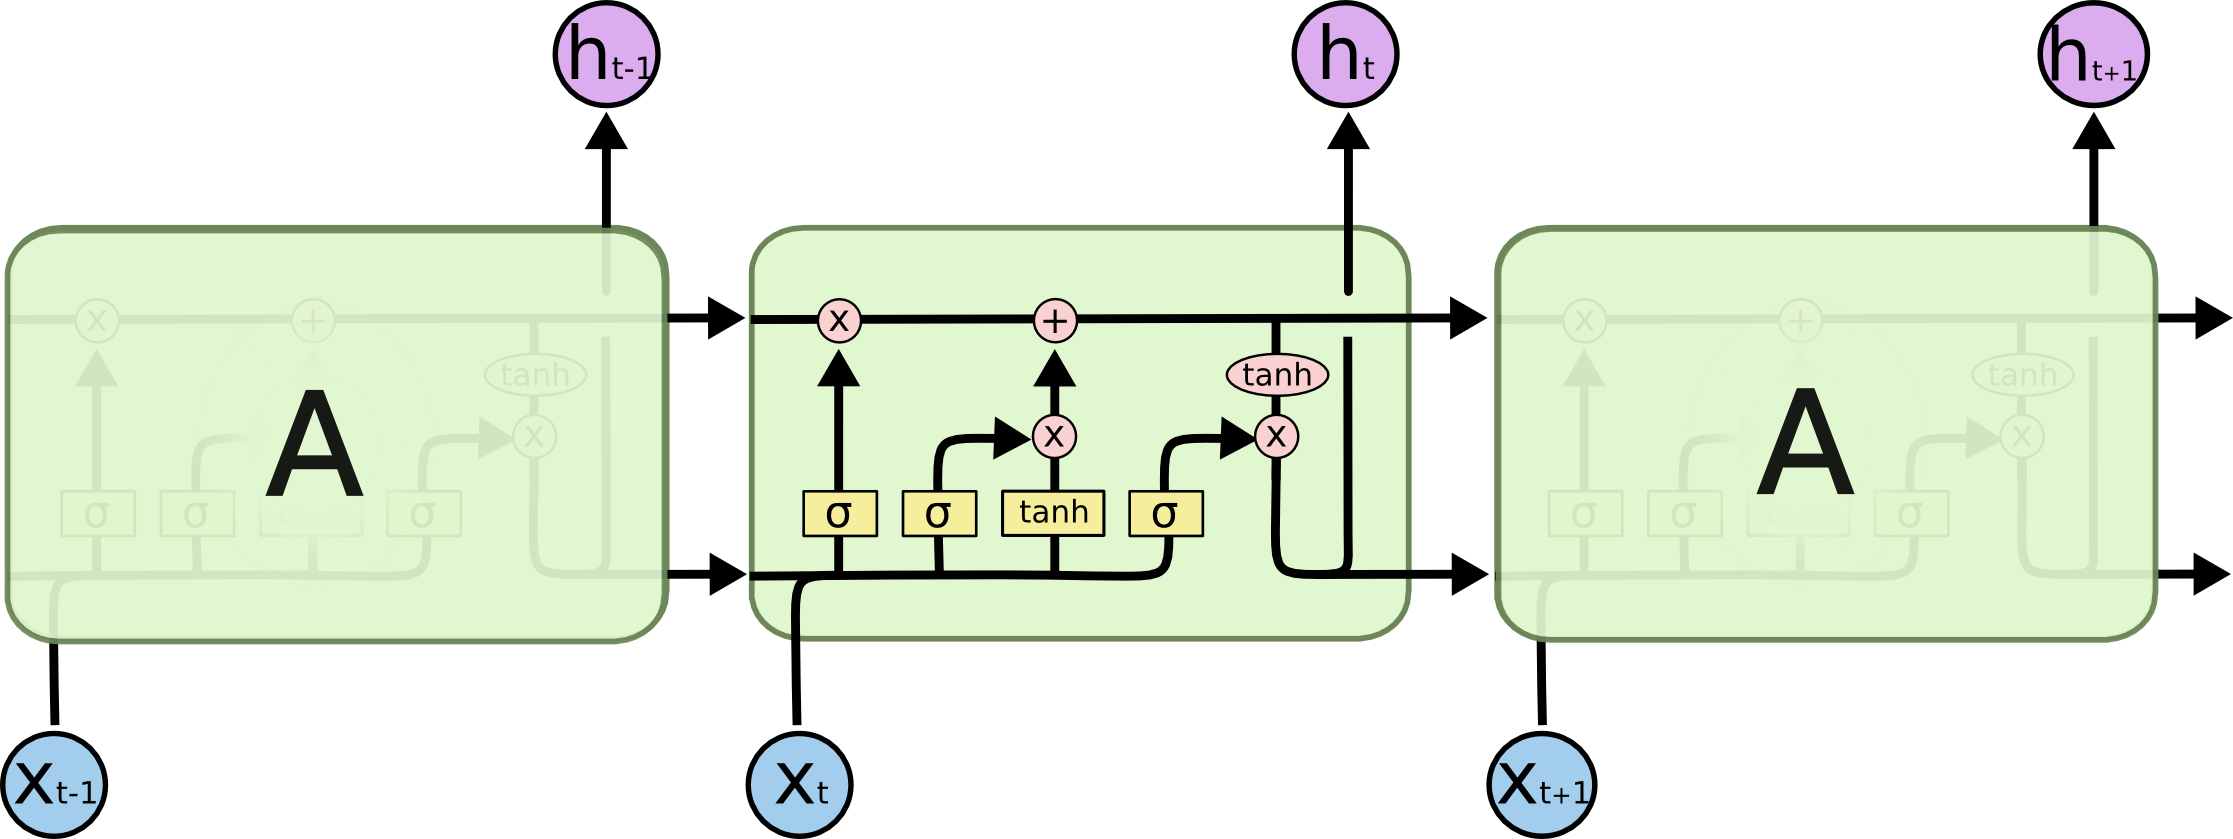
\includegraphics[width=\columnwidth]{figures/LSTM3-chain.png}
	\caption{Struttura di una cella LSTM. \textit{fonte:}~\cite{lstmblog}.
\label{fig:lstm}}
\end{figure}

\subsection{Output Encoder}
L'output in uscita da questo encoder è in forma di un tensore monodimensionale, di dimensione fissata, contenente le caratteristiche principali che compongono un nome di dominio.

\todo{ampliare}

\newpage
\section{Decoder}
\label{decoder}
La struttura del decoder è lascamente una copia speculare dell'encoder. L'obiettivo principale è riuscire a ricampionare un dominio partendo da un tensore a domensione inferiore rispetto alla codifica fornita in input all'encoder.

La struttura di massima presenta come primo layer un \textit{repeat vector} che ripete il tensore di input per un numero di volte pari alla lunghezza massima di dominio, fissata in fase di codifica del dataset, formando così un tensore 3-dimensionale, dello stessa dimensione dei domini provenienti dal dataset. La sequenza così formata viene data in input ad un layer LSTM avente le identiche caratteristiche del layer LSTM presente all'interno dell'encoder. Successivamente la sequenza di emissioni in output dalla LSTM viene fornita ad due reti convoluzionali parallele identiche al quelle inserite all'interno dell'encoder. il risultato di tale operazione è un vettore di dimensione pari a dizionario di caratteri ammissibili per i domini, per ogni step della sequenza di caratteri che compone un dominio. In Figura~\ref{fig:decoder} viene mostrato lo schema di massima del \textit{decoder}.

\begin{figure}[p]
    \centering
	%\documentclass{standalone}
%\usepackage{tikz}
%
%\usetikzlibrary{shapes,arrows,fit,calc,positioning}
%\usetikzlibrary{backgrounds}
\tikzstyle{box} = [draw, rectangle, fill=white, rounded corners, thick, node distance=5em, text width=7em, text centered, minimum height=2.5em]
\tikzstyle{container} = [draw, rectangle, dashed, inner sep=1em, node distance=5em]
\tikzstyle{line} = [draw, thick, -latex']
%\begin{document}
\begin{tikzpicture}[auto]
	\node [box] (conv) {Convolution Layer};
%	\node [box, below of=conv] (batch) {Batch Normalization};
%	\node [box, below of=batch](leaky) {Leaky ReLU activation};
%	\node [box, below of=leaky](dropout) {Dropout};
	\node [box, below of=conv](pooling){Average Pooling};

	\node [box, right of=conv, node distance=12em] (conv2) {Convolution Layer};
%	\node [box, below of=conv2] (batch2) {Batch Normalization};
%	\node [box, below of=batch2](leaky2) {Leaky ReLU activation};
%	\node [box, below of=leaky2](dropout2) {Dropout};
	\node [box, below of=conv2](pooling2){Average Pooling};
	
	\node [draw=none, above of=conv](invis4){};
	\node [draw=none, above of=conv2](invis5){};
	\node [draw=none, fit=(invis4)(invis5)](invis6){};
	\coordinate[above of=invis6,node distance=3em](begin_enc);
	\coordinate[above of=begin_enc,node distance=3em](in);
	\node at (begin_enc.north) [above,node distance=0 and 0] (input){};
	\node at (in.north) [box] (lstm){LSTM};	
	\node [box, above of=lstm](repvec){Repeat Vector};
	\coordinate [above of=repvec, node distance=3em](in);
	\node at (in.north)[above, node distance=0 and 0](testo_in){Dominio Codificato};	
	
	\node [draw=none, below of=pooling](invis){};
	\node [draw=none, below of=pooling2](invis2){};
	\node [draw=none, fit=(invis)(invis2)](invis3){};
	
	\node[box,below of=invis3, node distance=3em](conc){Concatenation Layer};
	\node[box,below of=conc](regr){Multinomial Regression};
	\coordinate[below of=regr,node distance=3em](end_enc);
	\node at (end_enc.south) [below,node distance=0 and 0] (output){Dominio};
	
	% area tratteggiata
	\node [container, fit=(conv)(pooling)](cnn){};
	\node [container, fit=(conv2)(pooling2)](cnn2){};
	\node at (cnn.north west) [above right,node distance=0 and 0] {Convnet};
	\node at (cnn2.north east) [above left,node distance=0 and 0] {Convnet};
	%%%%

	%%% frecce
	\path [line] (conv) -- (pooling);
%	\path [line] (batch) -- (leaky);
%	\path [line] (leaky) -- (dropout);
%	\path [line] (dropout) -- (pooling);
	\path [line] (pooling) |- (conc);

	\path [line] (conv2) -- (pooling2);
%	\path [line] (batch2) -- (leaky2);
%	\path [line] (leaky2) -- (dropout2);
%	\path [line] (dropout2) -- (pooling2);
	\path [line] (pooling2) |- (conc);
	
	\path [line] (conc) -- (regr);
	\path [line] (regr) -- (end_enc);
	
	\path [line] (in) -- (repvec);
	\path [line] (repvec) -- (lstm);
	\draw (lstm) -- (begin_enc);
	\path [line] (begin_enc) -| (conv);
	\path [line] (begin_enc) -| (conv2);
\end{tikzpicture}
%\end{document}
	\caption{Struttura del \textit{decoder}.
\label{fig:decoder}}
\end{figure}

\subsection{Regressione Multinomiale}
Lo step finale del decoder è un livello \textit{dense} di tipo \textit{time-distributed} che agisce come \textit{regressore multinomiale}, in grado di eseguire classificazione in diverse classi (in questo caso una classe per ogni carattere possibile nel dizionario). Il regressore multinomiale utilizza un tipo di attivazione \textit{softmax}, definito dalla funzione:

\[\sigma(\mathbf{z})_j = \frac{e^{z_j}}{\sum_{k=1}^K e^{z_k}}\qquad  \text{per}\; j=1,\ldots,K. \] 

dove $k$ è la dimensione del vettore di input $\mathbf{z}$ mentre in uscita si ottiene un vettore $k$-dimensionale $\sigma(\mathbf{z})$ di valori compresi in un intervallo $\left(0,1\right)$. Grazie a tale attivazione sull'ultimo layer, l'output del decoder rappresenta una distribuzione multinomiale rispetto ai caratteri di ammissibili, per ogni step temporale che compone. 
Tale distribuzione può essere campionata in modo da ottenere di nuovo un vettore numerico di interi contenente i caratteri codificati all'interno del vocabolario di caratteri ammissibili per i domini. 

Per il campionamento è stato usata una funzione \textit{softmax} utilizzata nel campo dell'apprendimento per rinforzo~\cite{reinflearning}, definita come: 

\[P_t(a) = \frac{\exp(q_t(a)/\tau)}{\sum_{i=1}^n\exp(q_t(i)/\tau)} \text{,}\]

Dove il valore di\textit{ "azione"} $q_{t}(a)$ corrisponde alla "ricompensa" ottenuta per l'azione $a$ e $\tau$  è definito come parametro di \textit{"temperatura"}. Per alte \textit{"temperature"} ( $\tau \to \infty$ ), tutte le azioni hanno la stessa probabilità e più bassa la temperatura, più la "ricompensa" influisce sulla probabilità. Per basse tempeature ($\tau \to 0^{+}$), la probabilità di \textit{azione} con la ricompensa più alta tende ad 1. 

Tramite questa funzione è stato possibile mettere a a punto in fase sperimentale il campionamento dei domini dalla lo rappresentazione in forma di tensore alla rappresentazione testuale.

\newpage
\section{Generative Adversarial Network}
\label{ganintro}
La \textit{Generative Adversarial Network (abbr. GAN)} èun modello di rete neurale formata da due reti che competono l'una contro l'altra: un \textit{generatore} che cerca di creare dati sintetici basati sulla vera distribuzione, con l'aggiunta di rumore in input ed un \textit{discriminatore}, che riceve un campione e deve predire se appartiene al set reale o sintetico. Questo processo continua in forma di competizione tra le due reti, nella quale il discriminatore apprende in maniera sempre più accurata a distinguere i campioni ed il generatore apprende la costruzione di dati sintetici sempre più realistici. Notevole è la struttura della GAN, la quale rende particolarmente difficoltosa la fase di \textit{training}: a differenza di reti neurali più semplici, non è possibile fissare un minimo da ottimizzare. Normalmente si attua una di discesa del gradiente, la quale fornisce l'ottimo per la fase di training, mentre nel caso di GAN, ogni passo effettuato durante la discesa del gradiente causa un cambiamento nella conformazione superficie di discesa. La composizione della GAN fa si che sia necessario invece trovare un equilibrio tra le due forze in gioco, impersonate da discriminatore e generatore. In figura~\ref{fig:gan} si può vedere una struttura di massima di una GAN.

\begin{figure}[!bp]
    \centering
	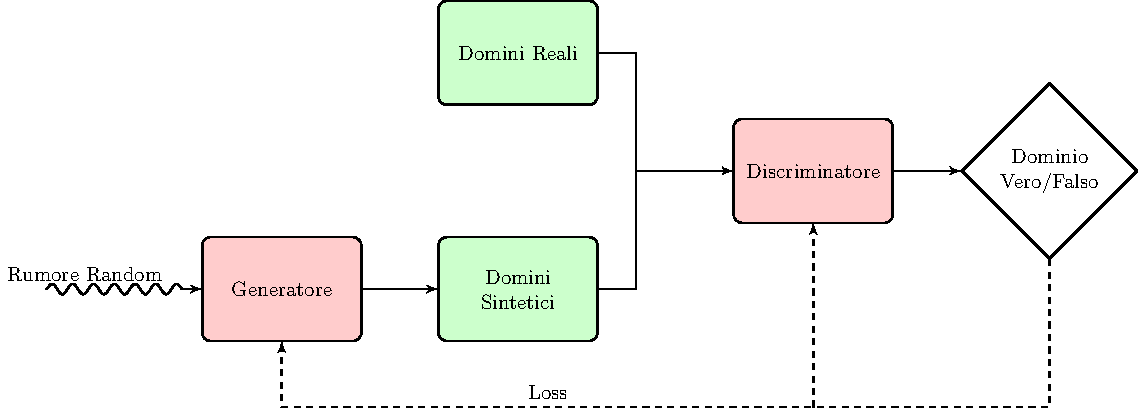
\includegraphics[width=\columnwidth]{figures/gan.tex}
	\caption{Struttura di una \textit{Generative Adversarial Network}.
\label{fig:gan}}
\end{figure}


La struttura dell'autoencoder descritto a partire dalla sezione~\ref{autoencoder} permette di produrre adeguatamente nomi di dominio che assomigliano a domini reali, ma in realtà sono generati pseudo-casualmente campionando le distribuzioni multinomiali in output all'autoencoder. Tuttavia l'uso di un autoencoder richiede la presenza di un ampio dataset di domini come input. Attraverso poche modifiche è stato possibile trasformare l'autoencoder in una \textit{GAN} che accetta in input un seme randomico ed emette nomi di dominio che appaiono simili ai domini reali.

\subsection{Architettura GAN}
\label{ganarch}
Come mostrato in figura~\ref{fig:archgan}, la struttura della GAN in esame è composta fondamentalmente dalle componenti dell'autoencoder, estese in modo da trasformare l'encoder in un discriminatore che possa classificare domini sintetici da domini reali, ed il decoder in un generatore che a partire da uno spazio latente possa generare domini codificati.

Rispetto al lavoro presentato in~\cite{deepdga}, si è deciso di implementare una architettura più semplificata. Come mostrato in~\cite{1606.03498} le GAN sono tipicamente difficoltose da allenare, in quanto l'uso di funzioni di costo porta ad un difficile \textit{tuning} per ottenere un equilibrio di Nash tra le due parti in gioco. La decisione finale è stata presa dopo una serie di test sperimentali, in cui si sono messe a confronto architetture similari comprendenti diverse conformazioni di layers atte ad rendere stabile la fase di training, tra le quali Batch Normalization, come mostrato in~\cite{1502.03167},  l'utilizzo di Leaky Relu~\cite{GANhacks} come layer di attivazione all'interno della sottorete Convoluzionale e Dropout come strumento per evitare il fenomeno di \textit{overfitting}~\cite{dropout}. L'uso di Leaky ReLU come funzione di attivazione è giustificata dalla riduzione della sparsità  del gradiente, la quale generalmente causa instabilità.

\begin{figure}[!htb]
    \centering
	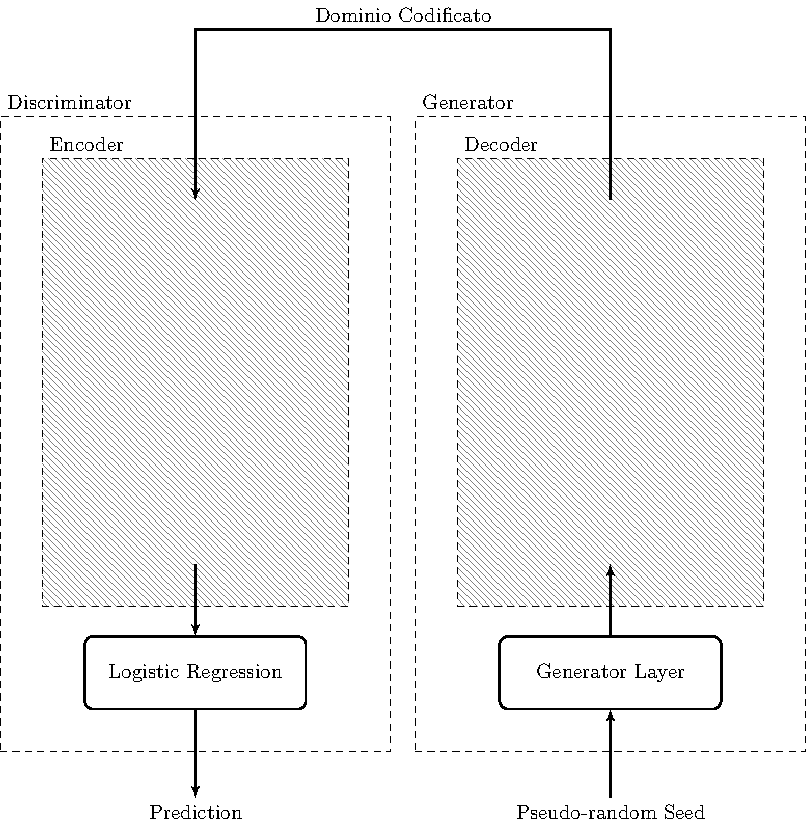
\includegraphics[width=\columnwidth]{figures/ganarch.tex}
	\caption{Struttura della GAN evoluta dell'autoencoder.
\label{fig:archgan}}
\end{figure}

\subsubsection{Batch Normalization}
L'utilizzo di Batch Normalization è stato introdotto per contrastare la nota difficoltà nel training delle GAN. Generalmente il training delle reti neurali è reso difficoltoso dal fatto che la distribuzione dell'input di ogni layer cambia durante il training così come cambiano i parametri dei precedenti layer. Questo fenomeno rallenta il training, richiedendo \textit{learning rates} più bassi ed una attenta scelta degli iperparametri iniziali. Tale fenomeno viene definito \textit{covariate shift} da~\cite{1502.03167}. Tramite l'uso di \textit{batch normalization} è possibile fare fronte a tali problematiche, le quali vengono amplificate grandemente dalla struttura avversaria delle due reti Generatore e Discriminatore che compongono la \textit{GAN}. 

\subsection{Generatore}
\label{generator}
Il generatore aggiunge in testa alla stuttura del decoder un layer denso che mappa un input randomico in una codifica di dominio, come mostrato in figura~\ref{fig:generator}. All'interno della sottorete convoluzionale è presente l'aggiunta di Batch Normalization, Leaky Relu al posto di ReLU per l'attivazione dei livelli convoluzionali.

Il Generator laye è formato da un generatore di rumore randomico di distribuzione gaussiana, la quale è stata provata come ottimale nel caso di GAN da~\cite{gaussian}. Tale distribuzione, di dimensione fissata, mima un possibile dominio codificato da encoder come descritto in sezione~\ref{encoder}. A partire da tale rumore è possibile per il decoder realizzare una codifica di dominio via via più realistica con l'avanzare delle epoche di training della GAN.

\begin{figure}[htbp]
    \centering
	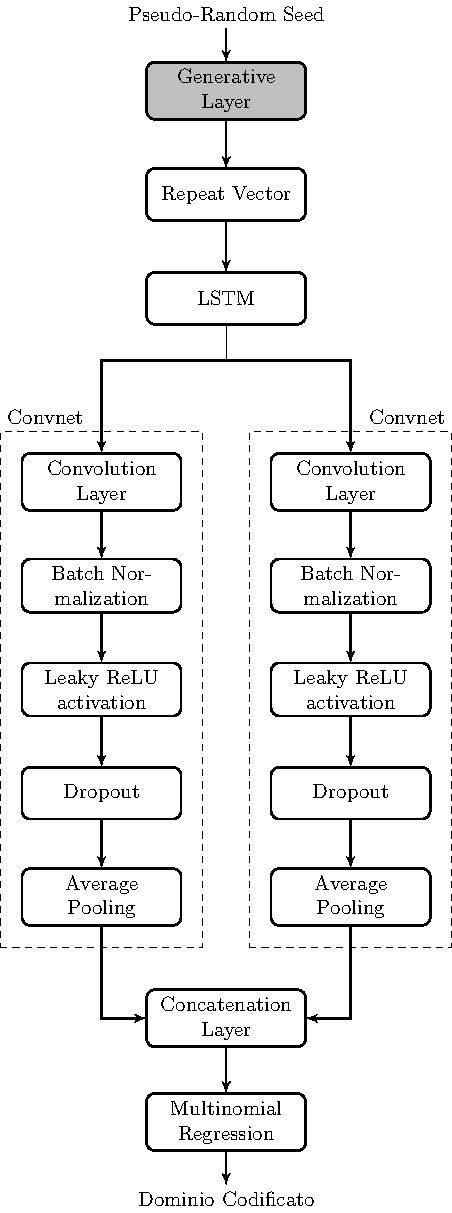
\includegraphics[width=\textwidth,height=\textheight,keepaspectratio]{figures/generator.tex}
	\caption{Struttura del generatore.
\label{fig:generator}}
\end{figure}

\subsection{Discriminatore}
\label{discriminator}
Il discriminatore implementa in uscita un layer denso che esegua regressione logistica sui domini codificati dalla sottorete encoder. ( Figura~\ref{fig:discriminator} ). Tale regressione viene attuata tramite un layer denso che effettua classificazione tra domini reali, codificati durante la fase di encoding attuata in~\ref{encoder}. La funzione di attivazione utilizzata all'interno del regressore logistico è la funzione sigmoide come descritto all'interno della sezione~\ref{classificatorenninterno}. Con il passare delle epoche di training, il discriminatore è sempre più in grado di distinguere domini reali da domini sintetici, forniti dal generatore. Tramite un insieme di tecniche sperimentali, è possibile evitare che il discriminatore prevalga sul generatore durante il training, mantenendo un equilibrio tra le due parti. 

\begin{figure}[htbp]
    \centering
	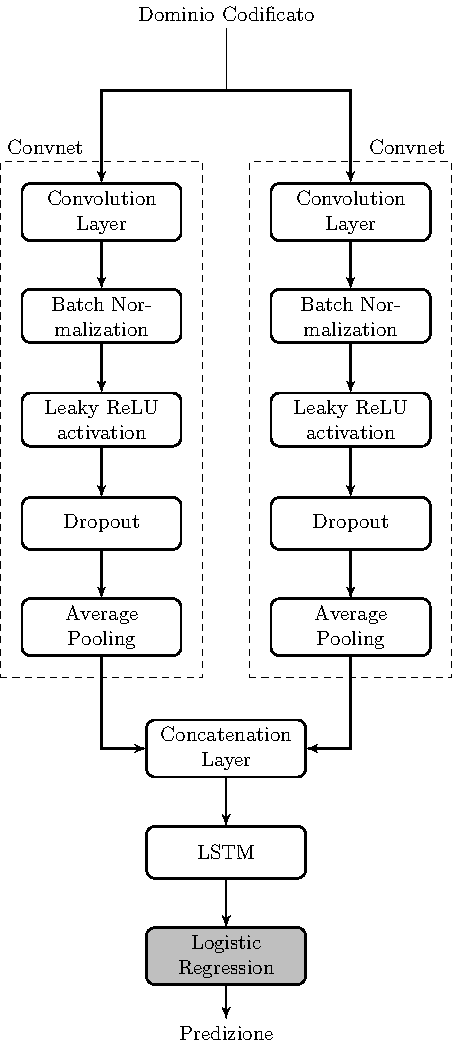
\includegraphics[width=0.5\columnwidth]{figures/discriminator.tex}
	\caption{Struttura del discriminatore.
\label{fig:discriminator}}
\end{figure}

\subsection{Funzionamento}
Durante la fase di training della GAN, il discriminatore ed il generatore vengono allenati in maniera concorrente. Per ogni step di training si estrae un subset fissato di domini dal dataset di domini reali e si genera un tensore di rumore generato randomicamente di lunghezza equivalente. Tale tensore viene dato in ingresso al generatore che restituisce una serie di domini sintetici codificati.

Successivamente il discriminatore viene allenato a distinguere i due subset estratti precedentemente, grazie ad un vettore di \textit{target} creato ad hoc, che identifica domini reali dai sintetici.

In ultima fase, i pesi del discriminatore vengono congelati e l'intero impianto della GAN viene allenato fornendo un nuovo tensore di rumore randomico ed un vettore di target ingannevoli, i quali identificano tutti i domini generati sinteticamente come reali. L'output di tale procedura è la funzione di loss del discriminatore, il quale non aggiorna la sua matrice di pesi durante questa fase. Tale funzione di loss indica quindi quanto "reali" sono stati i domini creati dal generatore.

Tramite questo espediente è possibile far si che la fase di training consista in fasi in cui il discriminatore impara a distinguere con più precisione domini reali da domini sintetici ed il generatore impari a fornire domini sintetici via via più realistici. Questa fase procede in maniera indefinita, fin tanto che l'equilibrio tra le due parti rimane tale.

